\documentclass[../report.tex]{subfiles}
\begin{document}
\graphicspath{{img/}{../img/}}
\section{Context awareness}
\label{sec:Context awareness}
To be able to make a context-aware framework, we first had to investigate what context and context-awareness is in a computer science perspective.

Context-awareness is a term associated with Ubiquitous computing. Ubiquitous computing, ubicomp, was coined in the early nineties by Mark Weiser whose vision was to make technology that could seamlessly assist in everyday tasks. Weiser's research-unit at Xerox PARC developed some of the first mobile devices, and the development of ubi computing clearly reflects in todays technology boom of smart phones and tablets.

\begin{quote}
\textit{``We have found two issues of crucial importance: location and scale. Little is more basic to human perception that physical juxtaposition, and so ubiquitous computers must know where they are. (Today's computers, in contrast, have no idea of their location and surroundings.) If a computer knows merely what room it is in, it can adapt its behavior in significant ways without requiring even a hint of artificial intelligence.''} Mark Wiser (1991) \cite{Mark Weiser (1991)}
\end{quote} 


As Weiser and his research team realised: For a system to weave itself into the everyday life to seamlessly interact with humans, the system must acquire knowledge to the current situation or \textit{context}. To make succeeding Ubiquitous computers, information of the surrounding environment is essential. Context-awareness provides environmental information, \textit{context-information}, to applications so that they can adapt a behaviour suitable to the current \textit{context}. Many of the publications on the subject describe context differently, but the one description fitting best our understanding was coined by Dey and Abowd whom described context as:

\begin{quote}
\textit{``Any information that can be used to characterize the situation of an entity. An entity is a person, place or object that is considered relevant to the interaction between a user and an application, including the user and application themselves.''} \cite{Dey and Abowd (2000)}
\end{quote} 

 


The holy grail of context-awareness is to understand and perform human intent, but it's important to keep in mind how difficult human intent is to understand. A person himself might event experience wonder at his own intentions. When humans interact, they can interpret the ongoing situation from the implicit understanding of body language, tone of voice, the surrounding environment as well as previous relations and information about past and future events. These \textit{context informations} are essential factors in effective communication.

Human-to-human interaction is, although the tremendous amount of context-information involved, never perfect and factors like culture differences have thought us the importance of knowledge in understanding intentions. The same goes for human-machine interactions where it seems a large amount of context-information, along with the ability to interpret it, is necessary for a machine to understand complex human intentions.


%As with most research, context-awareness is intended as a help in human life, be it direct or more indirect human-machine interaction. The holy grail is to understand and perform human intent, but it is important to remember that this is not even guaranteed in human-human interaction - A person himself might even have experienced wonder at his own intentions. Culture differences in human-human interactions have taught us the importance of knowledge in understanding intentions. The same goes for human-machine interaction where it seems a large amount of context-information is necessary for a machine to understand complex human intentions.

This said, not only increasing the available amount of context-information, but also heightening the quality and correctness of the information is important. As the amount of context increases, the context-aware application becomes able to take actions without explicit user input. When doing so, action can be taken on wrong or typically incomplete snaps of context. 


\begin{quote}
\textit{``Intelligibility and control are important user concerns in context-aware applications. They allow a user to understand why an application is behaving a certain way, and to change its behaviour.''} \cite{Dey and Newberger (2009)}
\end{quote} 

The above cited article stresses that insight to why an implicit action is carried out is important, and that it is important to offer the user to override this action. This brings us back to the previous discussed topic of understanding human intent. Computers will never fully understand human intent and therefore it is important to understand when implicit actions might be erroneous and the user therefore should be prompted before the action or have the ability to change the state back again.

\section{Context aware frameworks}
To support application developers a number of context-frameworks have been developed, for example JCAF and Context toolkit. When looking at previously developed frameworks mainly two approaches were used: Blackboard and Widget-based architecture \cite{Context-aware computing (2010)}

The blackboard approach is a centralized solution. Sensors and applications are connected to the blackboard and whenever a new sensor state is available a post-it, an entry to the database, is put on the blackboard. The application can at will look through the blackboard and search for context it might find relevant. The blackboard abstracts away the sensor implementation allowing the client to focus on only the context information. 

\begin{figure}
\centering
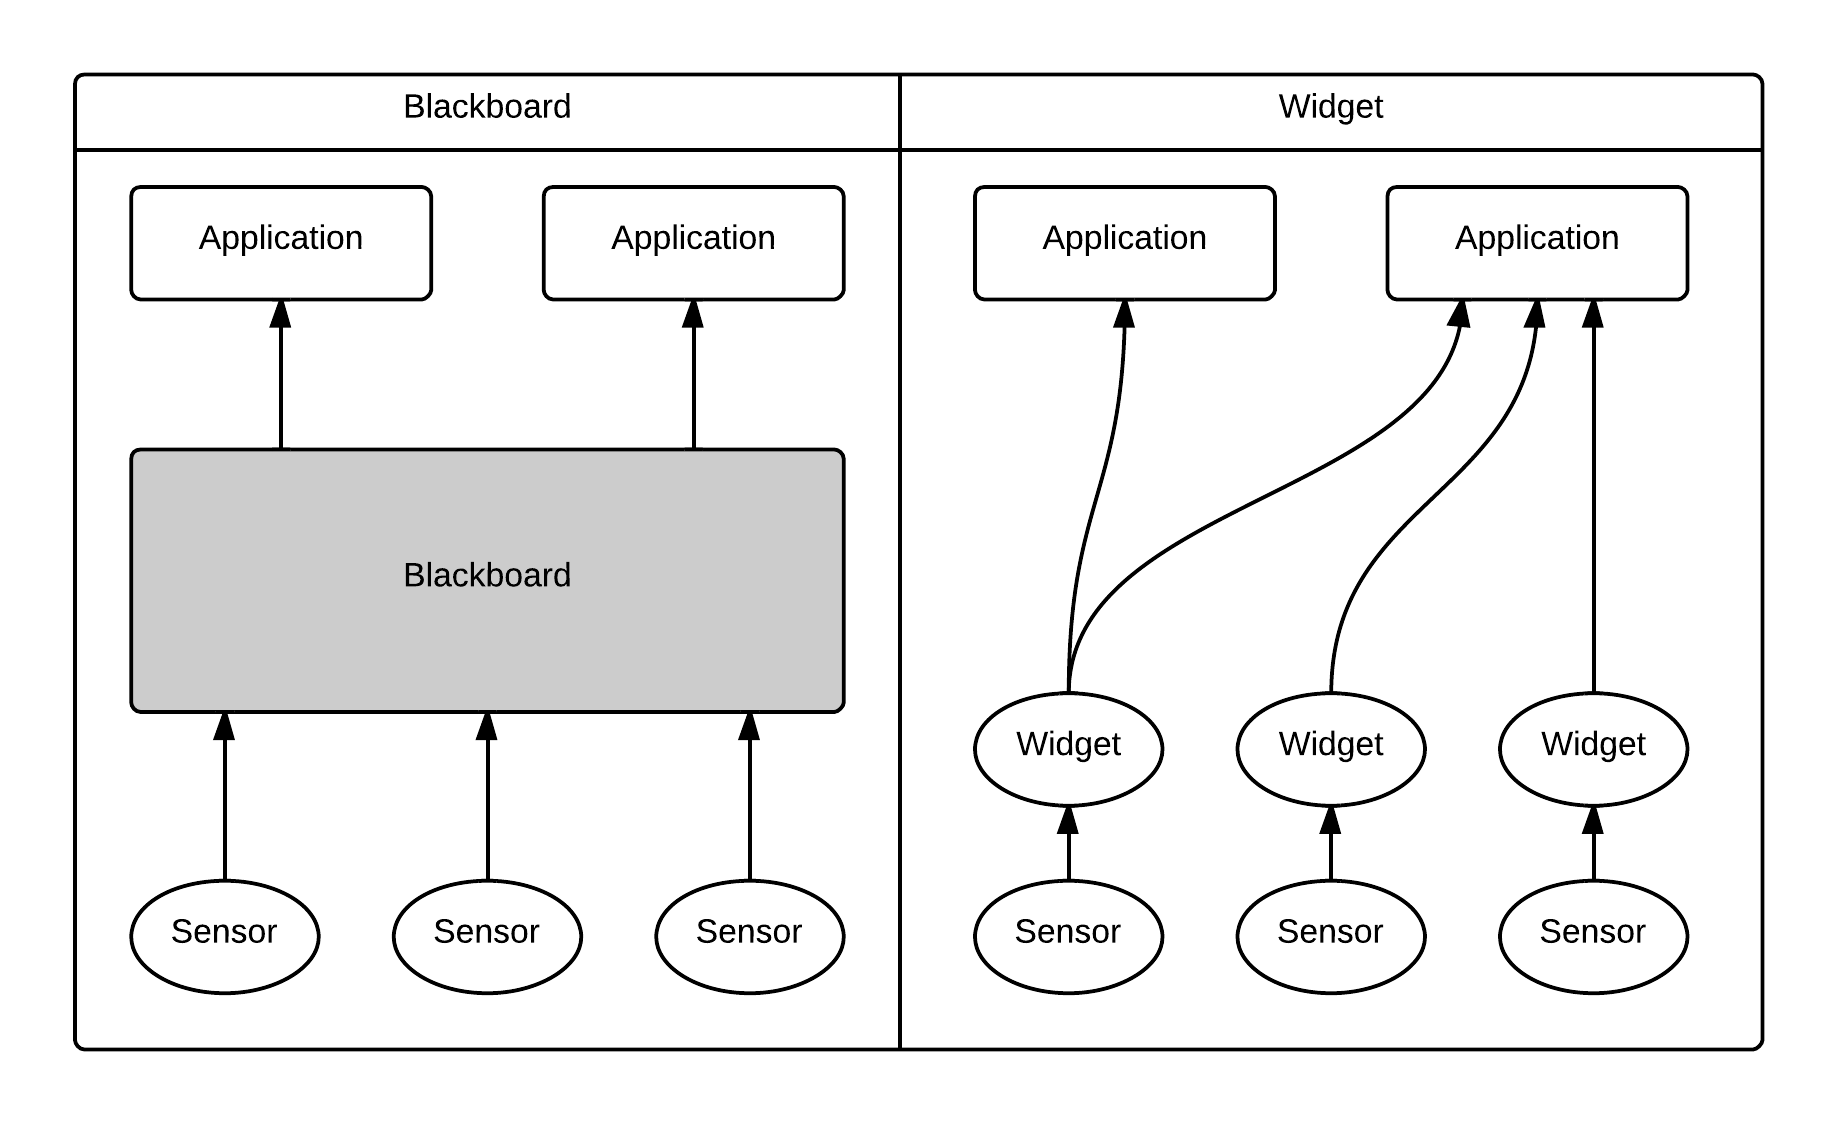
\includegraphics[width=\linewidth]{blackboard-widget.png}
\caption{Blackboard and widget-based approach}
\label{fig:blackboard-widget}
\end{figure}



The widget approach is an object-oriented distributed solution. Sensors encapsulated by widgets are available for application subscription. The solution is event based and applications are notified whenever a change to the sensor is occurring. This solution is object-oriented as the context is modelled with objects sent from sensor to application. This time and space coupled solution stands in contrast to the blackboard approach which have a database and is therefore time- and space uncoupled.

The solutions differs a lot in the way of modelling context, but the main difference is in the way of delivering context from sensor to application. The solutions stands in great contrast when looking at space and time coupling. To briefly describe the theory, space coupling is weather or not the sender knows who the receiver of a message is. Time coupling is if the given message is only available in real-time. 

Where the blackboard at any time offers applications to go though it's context database, it does not offer notifying the application, as the blackboard is space uncoupled, and does not know about the application. The widget solution offers live updated only when they happens and only to the applications subscribing for the update.

Both solutions are very useful in different applications.

For example a hospital system where you want to use the context framework to track patients, the blackboard solution seams to meet requirements best as you can, when needed, look up a patients whereabouts in the hospital.
This example requires lookup and for all information to be gathered in one place, supported by the blackboards time uncoupling and centralization. The traditional blackboard solution does on the other hand not support to warn for example the closest employee if a patient is trying to escape the premises which would be very useful.

For a home automation system using sensors, sensor input is only interesting the moment it happens, and only to actuator whom it concern. When a person enters the room the light should go on instantly, only in the room where the person entered and only at the given time. This example needs the time and space coupling supported by the widget and would not be doable with the tradition blackboard architecture.


\end{document}